% A.D.A.P.T. manuscript. Drafted with IEEEtran (journal mode) for compilation and review.
% Primary target: IEEE Access (original research article). Before submission, port the body to the official
% IEEE Access LaTeX template (https://ieeeaccess.ieee.org/authors/preparing-your-article/); see README.md.
\documentclass[journal]{IEEEtran}

\usepackage[T1]{fontenc}
\usepackage{cite}
\usepackage{amsmath,amssymb}
\usepackage{graphicx}
\usepackage{booktabs}
\usepackage{multirow}
\usepackage{array}
\usepackage{xcolor}
\usepackage{algorithm}
\usepackage{algorithmic}
\usepackage{tikz}
\usetikzlibrary{arrows.meta,positioning,fit,calc,shapes.geometric}
\usepackage{url}
\usepackage[hidelinks]{hyperref}

\newcommand{\adapt}{A.D.A.P.T.}
\newcommand{\yes}{\checkmark}
\newcommand{\part}{(\checkmark)}
\newcommand{\no}{--}
\renewcommand{\algorithmicrequire}{\textbf{Input:}}
\renewcommand{\algorithmicensure}{\textbf{Output:}}
% Empty frame reserved for a screenshot the authors will take from their own simulation run.
% #1: placeholder tag, #2: width, #3: height. Replace the whole \simplaceholder{...} by \includegraphics.
\newcommand{\simplaceholder}[3]{\fbox{\parbox[c][#3][c]{#2}{\centering\footnotesize\textbf{[FIGURE PLACEHOLDER --- #1]}\\[3pt]\scriptsize image to be inserted by the authors from their own simulation run}}}

\begin{document}

\title{A.D.A.P.T.: A Weather-Informed, Verifiable Pipeline from Annotated Flood Maps to Executable UAV Relief Missions}

\author{[Author~1], [Author~2], and [Faculty~Advisor]%
  \thanks{Manuscript draft prepared October 2026. [Funding statement: to be provided by the authors.]}%
  \thanks{The authors are with [Department], [Institution], [City], [Country] (e-mail: [corresponding.author@institution.edu]).}%
}

\markboth{Draft manuscript --- not peer reviewed}{[Author~1] \MakeLowercase{\textit{et al.}}: A.D.A.P.T.}

\maketitle

\begin{abstract}
Planning uncrewed aerial vehicle (UAV) relief flights after a flood requires an operator to read a flood map, choose delivery points, route around water and author an autopilot mission by hand. Prior work seldom produces a mission that an autopilot can load. This paper presents \adapt{}, an open pipeline that converts a flood-annotated map raster and current weather into QGroundControl WPL~110 missions. It combines operator-sampled HSV segmentation, a weather-parameterised flood-spread rule, per-region drop points, nearest-neighbour ordering, per-leg D*~Lite planning and a checked pixel-to-geodetic conversion. It supports two approaches: one drone visits every drop point, or a fleet of up to $K$ drones is used, in which each drone serves the cluster of drop points nearest its own base under a battery model. Fleet plans whose routes cross are rejected. On three published flood maps with a deterministic simulated operator, every generated mission passes an independent validator. Randomised coordinate round trips agree within $7\times10^{-8}$~px, and 31 of 33 injected defects are detected. Raising $K$ from 1 to 4 increases the drops served from 10 to 18 of 22 and from 17 to 34 of 41 under moderate weather. Limitations remain. Predicted-flood obstacles cause all 14 no-path legs of the single-UAV mode, one thematic map is segmented as 83\% flood, the multi-base assignment does not balance workload, and the maps are not georeferenced. No ground-station, simulation or flight validation has been performed, so \adapt{} is a verified research baseline, not a deployable system.
\end{abstract}

\begin{IEEEkeywords}
Unmanned aerial vehicles, disaster response, flood mapping, mission planning, multi-UAV planning, path planning, D* Lite, geospatial transformation, software verification.
\end{IEEEkeywords}


\section{Introduction}
\label{sec:intro}

\IEEEPARstart{F}{loods} disrupt road access exactly when isolated communities need supplies most. Small uncrewed aerial vehicles (UAVs) can reach such locations quickly and cheaply, and the disaster-management literature repeatedly identifies mapping, situational awareness and the delivery of small, urgent payloads as their most promising roles \cite{erdelj2017help,mohddaud2022applications,khan2022emerging,rejeb2021humanitarian}. Flood extents are now routinely produced from satellite and aerial data \cite{twele2016sentinel,bonafilia2020sen1floods11,rahnemoonfar2021floodnet} and are widely published as annotated maps. Turning such a map into a flight plan, however, is still largely a manual task: an operator must decide where packages can be dropped, in which order to visit those points, how to route around water, and how to encode the result in the mission format of an autopilot.

Each of these steps has a mature research literature, but the steps are usually studied in isolation. Flood segmentation methods stop at a mask \cite{gebrehiwot2019deep,simantiris2024unsupervised}; flood inundation models require digital elevation models and hydraulic forcing \cite{bates2000simple,ghimire2013formulation,teng2017flood}; relief-logistics models assume that demand locations are already known nodes in a graph \cite{otto2018optimization,rabta2018drone,dong2026path}; and path planners assume that an obstacle map is given \cite{aggarwal2020path,koenig2005fast}. A recent review of adaptive mission planning in emergencies observes that methods coupling hazard evolution, observation and mission planning remain fragmented across application domains \cite{gioia2026perspective}. Weather adds a further dynamic constraint, both on whether a drone can fly at all \cite{gao2021weather} and on how a flood may evolve.

\subsection{Problem Statement and Research Question}
Given a single flood-annotated map raster, a geographic reference and the current weather, the task is to produce, without training data or terrain models, a UAV mission that (i) visits one accessible delivery point for every flooded region, (ii) avoids current and near-term flooded areas where possible, (iii) releases a payload at each point, and (iv) can be loaded by a MAVLink-based ground station. When several UAVs are available, the same task is to distribute the delivery points among vehicles operating from separate launch bases, so that every vehicle's sorties fit its battery and payload and the vehicles' routes do not cross. The research question of this paper is therefore: \emph{to what extent can a lightweight, training-free pipeline convert an annotated flood map and current weather into an executable and verifiably correct UAV relief mission, and which limitations prevent such a mission from being geographically and operationally trustworthy?}

\subsection{Two Planning Approaches}
\adapt{} offers two ways of serving the same set of delivery points (Fig.~\ref{fig:modes}).
\begin{itemize}
\item \emph{Approach A: one drone.} A single UAV takes off from one home point, visits every delivery point in one tour and returns. This is the single-UAV mode (Section~\ref{sec:method}).
\item \emph{Approach B: a fleet of drones.} Up to $K$ UAVs operate from separate launch bases. The planner places the fewest bases that can reach the delivery points within battery range, then gives every delivery point to the nearest base that can serve it. Each drone therefore serves the cluster of flood regions around its own base, flying as many battery-limited sorties as it needs. This is the multi-base mode (Section~\ref{sec:multi}).
\end{itemize}
With $K=1$ the same planner produces a one-drone mission, which allows a like-for-like comparison of the two approaches (Section~\ref{sec:multires}). Approach B resembles what is often called a drone swarm, but in \adapt{} the drones are coordinated only before flight. The planner divides the work and checks that the routes do not cross; the drones do not communicate or adapt to each other while flying.

\subsection{Objectives}
The objectives are to (O1) describe and formalise every stage of an existing open implementation, \adapt{}, exactly as implemented; (O2) verify the correctness of its geospatial and mission-generation layers independently of the implementation; (O3) characterise its behaviour on real published flood maps, including ablation, sensitivity, optimality and baseline comparisons, and compare single- and multi-UAV planning on identical missions; and (O4) state explicitly what the evidence does and does not establish.

\subsection{Contributions}
The contributions are deliberately limited to what the implementation and its evaluation support:
\begin{enumerate}
\item \textbf{An integrated image-to-mission pipeline.} \adapt{} chains colour-based flood extraction, a weather-parameterised obstacle-inflation rule, boundary drop-point selection, nearest-neighbour ordering, per-leg D*~Lite planning and pixel-to-geodetic conversion into a QGroundControl WPL~110 mission with explicit payload-release commands (Sections~\ref{sec:arch}--\ref{sec:method}). The individual algorithms are established; the contribution is their integration and the resulting executable artefact.
\item \textbf{A single-drone and a drone-fleet approach.} Besides the single-UAV pipeline, a multi-base mode works as follows (Section~\ref{sec:multi}): it selects launch bases, gives each drone the cluster of delivery points nearest its base under a battery and payload model, plans one mission per drone and rejects plans whose routes cross. A controlled comparison on identical missions isolates the effect of the number of vehicles. The mode is a pre-flight planner with a nearest-feasible assignment, not a cooperative swarm.
\item \textbf{A precise formulation with stated validity domains.} Each stage is specified as implemented, including the failure behaviour of the planner and the conditions under which the geodetic conversion refuses to produce a coordinate (Section~\ref{sec:method}).
\item \textbf{A verification methodology for the geospatial and mission layers.} An independent WGS84 oracle, a specification-based mission validator that is itself tested against corrupted files, metamorphic resize tests and mutation testing are used to establish software correctness separately from geographic validity (Sections~\ref{sec:verif} and~\ref{sec:results}).
\item \textbf{An empirical characterisation that reports unfavourable outcomes.} On three published flood maps we report end-to-end behaviour, an ablation of predicted-flood obstacles, threshold sensitivity, the optimality gap of the route ordering, a planner baseline and a single- versus multi-UAV comparison, including failure modes (Section~\ref{sec:results}).
\end{enumerate}
We do not claim real-time operation, geographic accuracy for the supplied maps, flood-prediction accuracy, or simulated or physical flight validation; Section~\ref{sec:limits} discusses why.

The remainder of the paper is organised as follows. Section~\ref{sec:related} reviews related work and derives the gap. Section~\ref{sec:arch} formalises the problem and the architecture, Section~\ref{sec:method} details the single-UAV methodology, and Section~\ref{sec:multi} describes the multi-UAV mode. Section~\ref{sec:results} presents the experimental setup and results. Section~\ref{sec:limits} discusses limitations, threats to validity and safety. Section~\ref{sec:compare} positions \adapt{} relative to prior work, Section~\ref{sec:future} outlines future work, and Section~\ref{sec:conclusion} concludes.

\section{Related Work}
\label{sec:related}

\subsection{UAVs in Disaster Response}
Surveys of UAV use in disasters converge on three roles: rapid mapping and damage assessment, communication support, and delivery of small, time-critical payloads \cite{erdelj2017help,mohddaud2022applications,khan2022emerging}. Erdelj \emph{et al.} \cite{erdelj2017help} frame these roles across the prediction, assessment and response phases, and humanitarian-logistics reviews confirm that delivery to areas cut off by floods is a recurring motivation \cite{rejeb2021humanitarian}. Most of this literature is either conceptual or concerned with networking and coordination; for example, multi-UAV search-and-rescue frameworks address task allocation among vehicles \cite{alotaibi2019lsar}, and recent flood-management work simulates UAV-cluster deployment and resource scheduling with edge computing \cite{li2025urban}. Gioia \emph{et al.} \cite{gioia2026perspective} review adaptive mission planning and hazard monitoring for wildfires, chemical releases and floods, and identify the integration of hazard-evolution models with mission planning as fragmented across domains. These works motivate the problem but do not provide a path from a flood map to a mission file.

\subsection{Flood Mapping and Segmentation}
Classical water mapping relies on spectral indices such as the NDWI \cite{mcfeeters1996ndwi} and, for all-weather operation, on synthetic aperture radar with automated thresholding chains \cite{twele2016sentinel}. Learning-based methods require labelled data; Sen1Floods11 provides a georeferenced benchmark for Sentinel-1 \cite{bonafilia2020sen1floods11}, and FloodNet provides pixel-labelled post-flood UAV imagery \cite{rahnemoonfar2021floodnet}. Convolutional networks have been applied to UAV flood-extent mapping \cite{gebrehiwot2019deep}. Training-free colour-based methods remain attractive where labels are unavailable: Simantiris and Panagiotakis \cite{simantiris2024unsupervised} combine LAB-colour masks, a vegetation index and edges for unsupervised flood segmentation of UAV photographs, and Ibrahim \emph{et al.} \cite{ibrahim2021application} compare RGB/HSI clustering and region growing. All of these methods terminate at a flood mask; none produces delivery points or a flight plan. \adapt{} addresses a narrower perception problem than these works: it extracts flood pixels from \emph{already annotated} map products by operator-sampled HSV thresholding \cite{smith1978color}, followed by mathematical morphology \cite{haralick1987image} and border-following contour extraction \cite{suzuki1985topological}.

\subsection{Flood Modelling and Prediction}
Physically based and simplified inundation models range from raster storage-cell schemes such as LISFLOOD-FP \cite{bates2000simple} to cellular-automata (CA) models that replace the shallow-water equations by local transition rules on a digital elevation model \cite{ghimire2013formulation,guidolin2016weighted,jamali2019cellular}. CA models trade some accuracy for large speed-ups, but still require terrain data, rainfall or inflow forcing and calibration; Jamali \emph{et al.} \cite{jamali2019cellular} also report weaker performance where flow momentum matters. Teng \emph{et al.} \cite{teng2017flood} review this spectrum and its uncertainties. No reviewed model is coupled to UAV mission planning. The spread rule in \adapt{} is not a hydrological model: it is a terrain-free morphological proxy that dilates and shifts the observed mask according to precipitation and wind, and it is used only to inflate obstacles.

\subsection{Path Planning}
Grid search with A* \cite{hart1968formal} is optimal for static maps. Incremental methods, D* \cite{stentz1994optimal} and its simpler successor D*~Lite \cite{koenig2002dstar,koenig2005fast}, reuse search effort when edge costs change, which is valuable when a vehicle discovers obstacles during execution. Reviews of UAV path planning \cite{aggarwal2020path} catalogue classical, sampling-based and learning-based planners; they assume that the obstacle representation is given. \adapt{} uses D*~Lite on a downsampled occupancy grid derived from current and predicted flood masks; as shown in Section~\ref{sec:results}, its present offline use does not exercise the incremental property.

\subsection{Route Optimisation and Relief Logistics}
Visiting a set of delivery points is a travelling-salesman-type problem. Exact dynamic programming is exponential \cite{held1962dynamic}, and the nearest-neighbour construction heuristic can be a logarithmic factor worse than optimal in the worst case \cite{rosenkrantz1977analysis}. Operations-research work on UAV delivery formulates truck--drone tandems \cite{murray2015flying} and drone fleets for last-mile relief \cite{rabta2018drone}; Otto \emph{et al.} \cite{otto2018optimization} survey this area. Most closely related, Dong \emph{et al.} \cite{dong2026path} optimise multi-vehicle, multi-UAV flood-rescue delivery with flood-depth-dependent road speeds using mixed-integer programming and adaptive large-neighbourhood search. These models are more rigorous than \adapt{}'s ordering heuristic, but take demand locations and network states as given inputs rather than deriving them from imagery, and output schedules rather than autopilot missions.

\subsection{Landing and Drop-Site Selection}
Image-based selection of safe landing zones has been studied using multichannel imagery fused with map data \cite{patterson2014timely} and texture-based flat-surface detection \cite{kaljahi2019automatic}. These methods score candidate sites for landing safety. \adapt{} has no comparable safety model: its ``safe'' drop point is a convex-hull vertex on the boundary of a flood region, chosen for accessibility from the route, without terrain, population or obstacle information.

\subsection{Mission Generation and Geospatial Conversion}
MAVLink is the de facto protocol between ground stations and open autopilots \cite{meier2012pixhawk,koubaa2019micro}; missions are commonly exchanged as QGroundControl WPL plain-text files \cite{mavlink_fileformat} whose command semantics are defined by the common message set \cite{mavlink_common} and refined per autopilot \cite{ardupilot_missioncmds,px4_missions}. Converting image coordinates to geodetic coordinates requires a projection model \cite{snyder1987map}; web-map imagery uses Web Mercator, whose scale varies with latitude \cite{battersby2014implications}, and accurate geodesics on the ellipsoid are available from Vincenty's and Karney's algorithms \cite{vincenty1975direct,karney2013algorithms}. We found no reviewed work that generates WPL missions from flood imagery and verifies the geodetic and mission layers.

\subsection{Synthesis and Gap}
Table~\ref{tab:gap} summarises the capabilities reported by representative work. Perception, hazard modelling, path planning, route optimisation and site selection are each well developed, but in the reviewed literature they are rarely combined into a chain that starts from flood imagery and ends in an executable autopilot mission, and the correctness of the image-to-geodetic and mission-encoding steps is not reported. \adapt{} addresses this intersection with deliberately simple components. Its contribution is integration and verification; each of its components is weaker than the specialised state of the art in its own area.

\begin{table*}[t]
\centering
\caption{Capabilities reported by representative related work and by \adapt{}. \yes{}: addressed; \part{}: partially or under strong simplification; \no{}: not addressed in the cited work as reported. The table reflects the stated scope of each paper and is not exhaustive.}
\label{tab:gap}
\footnotesize
\setlength{\tabcolsep}{4pt}
\begin{tabular}{@{}p{4.9cm}cccccccc@{}}
\toprule
Work (group) & \shortstack{Flood\\perception} & \shortstack{Hazard\\evolution} & \shortstack{Weather\\input} & \shortstack{Obstacle-aware\\path planning} & \shortstack{Delivery-point\\selection} & \shortstack{Visit\\ordering} & \shortstack{Executable\\autopilot mission} & \shortstack{Geo/mission\\verification}\\
\midrule
Flood segmentation \cite{gebrehiwot2019deep,simantiris2024unsupervised,rahnemoonfar2021floodnet} & \yes & \no & \no & \no & \no & \no & \no & \no\\
SAR flood mapping \cite{twele2016sentinel,bonafilia2020sen1floods11} & \yes & \no & \no & \no & \no & \no & \no & \no\\
Inundation models \cite{bates2000simple,ghimire2013formulation,guidolin2016weighted,jamali2019cellular} & \no & \yes & \part & \no & \no & \no & \no & \no\\
Incremental grid planning \cite{stentz1994optimal,koenig2005fast} & \no & \no & \no & \yes & \no & \no & \no & \no\\
Relief / drone routing \cite{murray2015flying,rabta2018drone} & \no & \no & \no & \no & \no & \yes & \no & \no\\
Flood-rescue collaborative delivery \cite{dong2026path} & \no & \no & \no & \part & \no & \yes & \no & \no\\
Safe landing-zone detection \cite{patterson2014timely,kaljahi2019automatic} & \part & \no & \no & \no & \part & \no & \no & \no\\
Multi-UAV SAR / flood deployment \cite{alotaibi2019lsar,li2025urban} & \no & \no & \no & \part & \no & \yes & \no & \no\\
\midrule
\adapt{} (this work) & \part{}$^{a}$ & \part{}$^{b}$ & \yes{}$^{c}$ & \yes & \part{}$^{d}$ & \part{}$^{e}$ & \yes & \yes{}$^{f}$\\
\bottomrule
\end{tabular}\\[2pt]
\parbox{\textwidth}{\scriptsize $^{a}$Annotated map products only, operator-sampled colour thresholds. $^{b}$Terrain-free morphological proxy, uncalibrated. $^{c}$Current precipitation and wind only. $^{d}$Boundary geometry only, no safety model. $^{e}$Nearest-neighbour heuristic. $^{f}$Software verification only; no ground-station, SITL or flight validation.}
\end{table*}

\section{Problem Formulation and Architecture}
\label{sec:arch}

\subsection{Notation}
Let $I$ be the input raster of $W_0\times H_0$ pixels. If $W_0$ exceeds a display width $D$ (750~px by default), the image is resized to $I'$ of size $W'\times H'$ with $W'=D$, $H'=\operatorname{round}(H_0 s)$ and $s=D/W_0$; otherwise $I'=I$ and $s=1$. All perception and planning operate on the pixel domain $\Omega=\{0,\dots,W'-1\}\times\{0,\dots,H'-1\}$ of $I'$, with OpenCV conventions: $x$ is the column (increasing to the east of a north-up map) and $y$ the row (increasing to the south), and integer coordinates denote pixel centres.

The pipeline produces the following objects:
\begin{itemize}
\item a binary flood mask $M\subseteq\Omega$ extracted from $I'$;
\item weather $w=(P,V,\theta)$: precipitation $P$ (mm), wind speed $V$ (km/h) and meteorological wind direction $\theta$ (degrees, direction the wind blows \emph{from});
\item a predicted mask $\hat M\supseteq M$ after a horizon of $T$ hours, and an obstacle set $O=M\cup\hat M$;
\item flood regions $R_1,\dots,R_n$, the external contours of $M$ with area at least $a_{\min}$;
\item drop points $d_i\in\mathcal{V}(\operatorname{conv}R_i)$, one vertex of the convex hull of each region, and a HOME point $h\in\{d_i\}$;
\item a visiting order $\pi$ and a pixel route $P=(p_0,\dots,p_m)$ with $p_0=p_m=h$;
\item a mission $\mathcal{W}$, a sequence of MAVLink mission items with geodetic coordinates $(\varphi,\lambda)$ derived from a reference $(\varphi_0,\lambda_0)$ and a ground scale $\rho$ (METERS\_PER\_PIXEL, metres per \emph{original} pixel).
\end{itemize}

\subsection{Problem Statement}
Given $(I,w,\varphi_0,\lambda_0,\rho)$, produce $\mathcal{W}$ such that the vehicle takes off at $h$, visits every $d_i$ once at cruise altitude, descends and releases a payload at each $d_i$, avoids $O$ wherever a free path exists on the planning grid, and returns to $h$. \adapt{} does not solve this as a joint optimisation problem. It decomposes it into a fixed sequence of heuristic stages (Fig.~\ref{fig:architecture}), each of which is specified in Section~\ref{sec:method}. No optimality is claimed for the composition. In particular, visit ordering ignores obstacles, and path planning is optimal only per leg and on a coarse grid.

% Fig. 1: A.D.A.P.T. architecture (matches main.py call order; letters refer to Section IV subsections).
\begin{figure*}[t]
\centering
\begin{tikzpicture}[
  font=\scriptsize, node distance=3mm and 7.5mm,
  stage/.style={draw, rounded corners=1pt, align=center, minimum height=9mm, text width=20mm, fill=blue!6},
  io/.style={draw, align=center, minimum height=9mm, text width=20mm, fill=orange!12},
  ver/.style={draw, rounded corners=1pt, align=center, minimum height=7mm, text width=30mm, fill=green!7},
  lab/.style={font=\tiny, fill=white, inner sep=0.6pt},
  arr/.style={-{Stealth[length=1.6mm]}, semithick}]
  % row 1: perception and selection
  \node[io] (img) {flood-annotated\\map raster $I$};
  \node[stage, right=of img] (seg) {(A, B) display scaling,\\HSV sampling,\\morphology};
  \node[stage, right=of seg] (reg) {(C) contours,\\hulls, centroids};
  \node[stage, right=of reg] (drop) {(G) boundary drop\\points and HOME};
  \node[stage, right=of drop] (nn) {(H) nearest-\\neighbour order};
  \node[io, right=of nn] (cfg) {reference $(\varphi_0,\lambda_0)$,\\scale $\rho$};
  % row 2: environment, planning and output
  \node[io, below=11mm of img] (wx) {weather $(P,V,\theta)$\\(Open-Meteo or file)};
  \node[stage, right=of wx] (spread) {(D, E) weather-\\driven spread rule};
  \node[stage, right=of spread] (obs) {(F) obstacles\\$O=M\cup\hat M$};
  \node[stage, right=of obs] (dstar) {(I) per-leg D*~Lite\\on $5{\times}$ grid};
  \node[stage, right=of dstar] (geo) {(J) pixel-to-geodetic\\with validity checks};
  \node[io, right=of geo] (wpl) {(K) QGC WPL 110\\mission file};
  % data flow
  \draw[arr] (img) -- (seg);
  \draw[arr] (seg) -- node[lab, above=1pt]{$M$} (reg);
  \draw[arr] (reg) -- node[lab, above=1pt]{$R_i$} (drop);
  \draw[arr] (drop) -- node[lab, above=1pt]{$d_i, h$} (nn);
  \draw[arr] (wx) -- (spread);
  \draw[arr] (seg.south) -- node[lab, right=1pt, pos=0.45]{$M$} (spread.north);
  \draw[arr] (spread) -- node[lab, above=1pt]{$\hat M$} (obs);
  \draw[arr] (obs) -- node[lab, above=1pt]{$O$} (dstar);
  \draw[arr] (nn.south) -- node[lab, right=1pt, pos=0.45]{$\pi$} (dstar.north);
  \draw[arr] (dstar) -- node[lab, above=1pt]{$P$} (geo);
  \draw[arr] (cfg.south) -- (geo.north);
  \draw[arr] (geo) -- (wpl);
  % verification layer
  \node[ver, below=7mm of obs] (oracle) {independent WGS84 oracle\\(Vincenty) and round trips};
  \node[ver, right=6mm of oracle] (val) {specification-based\\WPL validator (tested)};
  \node[ver, right=6mm of val] (mut) {regression, metamorphic\\and mutation tests};
  \node[draw, dotted, inner sep=1.6mm, fit=(oracle)(val)(mut)] (vbox) {};
  \node[anchor=east, align=right, font=\scriptsize] at (vbox.west) {offline verification\\(Sec.~\ref{sec:verif})~};
  \draw[arr, dotted] (val.north) -- (geo.south);
  \draw[arr, dotted] (mut.north) -- (wpl.south);
\end{tikzpicture}
\caption{Architecture of \adapt{} as implemented. Letters refer to the subsections of Section~\ref{sec:method}. Blue boxes are pipeline stages executed in this order by the entry point; orange boxes are inputs and the output. The dotted block is the offline verification layer, which is not part of the run-time pipeline. Colour sampling is the only interactive step.}
\label{fig:architecture}
\end{figure*}


\subsection{Architecture and Interfaces}
Fig.~\ref{fig:architecture} shows the implemented data flow. The entry point validates its arguments and the geographic configuration before any work is done (Section~\ref{sec:geo}), then runs the stages in the order shown. The only interactive step is colour sampling, in which the operator clicks on flood pixels. The planner and the geodetic conversion are the only stages with explicit failure semantics:
\begin{itemize}
\item a leg with no free path is logged and flown as a straight segment;
\item a coordinate outside the conversion's validity domain aborts mission generation without writing a file.
\end{itemize}
A mission file left by an earlier run is removed once the input image has been loaded, so that a run which fails afterwards cannot leave an older mission that could be mistaken for its output. The implementation is written in Python using OpenCV \cite{bradski2000opencv} and NumPy, and is accompanied by an offline verification layer (Section~\ref{sec:verif}).

\section{Methodology}
\label{sec:method}

This section specifies each stage exactly as implemented in the evaluated version of \adapt{}. Parameter values are the defaults used in all experiments (Table~\ref{tab:config}).

\subsection{Input Acquisition and Display Scaling}
The input is a raster in which flooded areas have been drawn in a distinct colour (red in all evaluated maps). The image is decoded with OpenCV and, if wider than $D$, downscaled with area interpolation to $I'$ (Section~\ref{sec:arch}). Scaling serves interactive display; because every later stage works in display pixels, all pixel-unit parameters below have a ground size that depends on $s$. This is accounted for in the geodetic conversion (Section~\ref{sec:geo}) but not in the perception and planning parameters (Section~\ref{sec:limits}).

\subsection{Colour Sampling and Flood Segmentation}
The operator clicks $K$ flood pixels $c_k=(x_k,y_k)$ in $I'$. For each click, all pixels of the $11\times11$ patch $\Pi_k$ centred on $c_k$ (clipped at the image border) are converted to HSV \cite{smith1978color} with OpenCV's ranges $H\in[0,179]$, $S,V\in[0,255]$. Let $\mathcal{S}=\bigcup_k\mathrm{HSV}(I'(\Pi_k))$. Writing $C^{-}$ and $C^{+}$ for the minimum and maximum of channel $C$ over $\mathcal{S}$, the thresholds are the sample extrema widened by margins $\delta_H=20$ and $\delta_{SV}=30$:
\begin{align}
\ell_H&=\max(H^{-}-\delta_H,0),\quad u_H=\min(H^{+}+\delta_H,179),\label{eq:hsvH}\\
\ell_C&=\max(C^{-}-\delta_{SV},0),\quad u_C=\min(C^{+}+\delta_{SV},255),\label{eq:hsvSV}
\end{align}
for $C\in\{S,V\}$. Because red straddles the hue origin, a \emph{red-wrap} rule applies when $\ell_H\le10$ or $u_H\ge170$: the hue interval is then replaced by the fixed set $\mathcal{H}=[0,10]\cup[170,179]$ while the S and V intervals are kept; otherwise $\mathcal{H}=[\ell_H,u_H]$. The raw mask is
\begin{multline}
M_0=\{p\in\Omega:\,H(p)\in\mathcal{H},\\ S(p)\in[\ell_S,u_S],\ V(p)\in[\ell_V,u_V]\},
\end{multline}
and the flood mask is obtained by a morphological closing followed by an opening \cite{haralick1987image} with a $5\times5$ square structuring element $B$:
\begin{equation}
M=(M_0\bullet B)\circ B .
\label{eq:morph}
\end{equation}
Two properties follow directly from these definitions and matter for the results. First, whenever the red-wrap rule fires, as it does for every map evaluated here, $\delta_H$ has no effect on $M$. Second, the patch contains background pixels around small or thin markings, so $\ell_S$ can fall to $0$; since OpenCV assigns hue $0$ to achromatic (grey and white) pixels, white background can then satisfy all three conditions. Section~\ref{sec:results} shows both effects.

\subsection{Flood-Region Extraction}
External contours of $M$ are extracted by border following \cite{suzuki1985topological}, and contours with area below $a_{\min}=200$~px$^2$ are discarded. Each remaining region $R_i$ is represented by the vertex set of its convex hull and by its image-moment centroid $c_i=(\lfloor m_{10}/m_{00}\rfloor,\lfloor m_{01}/m_{00}\rfloor)$. Regions are taken from the current mask $M$ only; predicted flooding affects obstacles but creates no new delivery targets.

\subsection{Weather Acquisition}
\label{sec:weather}
Current conditions at $(\varphi_0,\lambda_0)$ are requested from the Open-Meteo forecast API \cite{zippenfenig2024openmeteo}: precipitation, 10-m wind speed, 10-m wind direction and visibility (the last is not used). Responses are cached per coordinate, and requests time out after 10~s. On any request or parsing failure a calm fallback $(P,V,\theta)=(0,0,0)$ is returned and a warning is logged. Note that Open-Meteo reports current-condition precipitation as a sum over the preceding reporting interval, for example 15~minutes \cite{openmeteo_docs}, whereas the spread rule below interprets $P$ per hour. Wind above 40~km/h and precipitation above 15~mm trigger warnings but do not stop the pipeline. For reproducibility, the experiments use a weather file with $(P,V,\theta)=(10~\text{mm},30~\text{km/h},270^\circ)$.

\subsection{Weather-Driven Spread Rule}
\label{sec:spread}
\adapt{} estimates near-term flood growth with a deterministic, terrain-free rule applied to the binary mask (Algorithm~\ref{alg:spread}). It can be read as a cellular automaton whose cells become flooded if any cell within an elliptical neighbourhood is flooded (isotropic growth), combined with a rigid advection of the flooded set in the downwind direction. With
\begin{equation}
b=\max(0,\lfloor P/5\rfloor),\ \ v=\max(0,\lfloor V/10\rfloor),\ \ \alpha=\theta+180^\circ,
\label{eq:spread}
\end{equation}
the shift is $(\Delta x,\Delta y)=(\operatorname{round}(v\sin\alpha),\operatorname{round}(-v\cos\alpha))$ display pixels, and $N=\max(1,\lfloor T\rfloor)$ iterations are applied. For the experimental weather, $b=2$, $v=3$, $\alpha=90^\circ$ (eastward), $(\Delta x,\Delta y)=(3,0)$ and $N=2$ for $T=2$~h. The rule has not been calibrated against observed flood evolution or compared with hydrodynamic models; its coefficients are documented in the code as heuristic. It is used only to make the planner keep clear of areas that may flood soon.

\begin{algorithm}[t]
\caption{Weather-driven spread rule (Stage E)}
\label{alg:spread}
\begin{algorithmic}[1]
\REQUIRE mask $M$, weather $(P,V,\theta)$, horizon $T$ (h)
\ENSURE predicted mask $\hat M\supseteq M$
\STATE $b\gets\max(0,\lfloor P/5\rfloor)$; $v\gets\max(0,\lfloor V/10\rfloor)$; $\alpha\gets\theta+180^\circ$
\STATE $\Delta x\gets\operatorname{round}(v\sin\alpha)$; $\Delta y\gets\operatorname{round}(-v\cos\alpha)$
\STATE $\hat M\gets M$
\FOR{$t=1$ \TO $\max(1,\lfloor T\rfloor)$}
  \IF{$b>0$} \STATE $\hat M\gets\hat M\oplus E_{2b+1}$ \COMMENT{dilation, elliptical element} \ENDIF
  \IF{$v>0$} \STATE $\hat M\gets\hat M\cup\tau_{(\Delta x,\Delta y)}(\hat M)$ \COMMENT{shift, zero fill} \ENDIF
\ENDFOR
\RETURN $\hat M$
\end{algorithmic}
\end{algorithm}

\subsection{Obstacle Modelling}
The obstacle set is $O=M\cup\hat M$, which equals $\hat M$ because the rule only adds pixels. Using $O$ rather than $M$ trades route exposure to predicted flooding against free-space connectivity; Section~\ref{sec:results} quantifies both sides of this trade-off.

\subsection{Drop-Point and HOME Selection}
For each region, one hull vertex is chosen as its drop point. Let $\Gamma$ be the polyline through the centroids $c_1,\dots,c_n$ in contour-discovery order. Then
\begin{equation}
d_i=\arg\min_{q\in\mathcal{V}(\operatorname{conv}R_i)}\ \min_{j}\operatorname{dist}\big(q,\overline{c_jc_{j+1}}\big),
\label{eq:drop}
\end{equation}
with the point-to-segment distance; for $n=1$ the first hull vertex is used. The drop point is therefore on the flood boundary, not inside the water. It is ``safe'' only in this geometric sense: no terrain, structure, population or landing-safety information is used, unlike dedicated site-selection methods \cite{patterson2014timely,kaljahi2019automatic}. $\Gamma$ joins centroids in discovery order, not in the final visiting order, and $O$ is not consulted. HOME is the drop point nearest to the integer image centre: $h=\arg\min_i\lVert d_i-(\lfloor W'/2\rfloor,\lfloor H'/2\rfloor)\rVert$. The region whose drop point becomes HOME still receives a delivery.

\subsection{Visit Ordering}
The visiting order is built by the nearest-neighbour heuristic: starting at $h$, the closest unvisited drop point in Euclidean pixel distance is appended until all are visited, and $h$ is appended at the end. Because $h$ is itself a drop point, the first step has zero length. The procedure is $O(n^2)$, ignores obstacles, and carries no optimality guarantee; its worst-case ratio to the optimal tour grows logarithmically with $n$ \cite{rosenkrantz1977analysis}. Section~\ref{sec:results} measures its gap empirically.

\subsection{Per-Leg Path Planning with D*~Lite}
\label{sec:dstar}
\emph{Grid.} $O$ is downsampled by a factor $f=5$ with nearest-neighbour resampling to an occupancy grid $G$ of $\lfloor W'/5\rfloor\times\lfloor H'/5\rfloor$ cells. Each cell therefore reflects a single sample of its $5\times5$ block, so features thinner than a cell can be missed.

\emph{Endpoints.} Consecutive stops $(p,q)$ are mapped to cells by integer division and clamped to the grid. Because drop points lie on flood boundaries, endpoints frequently fall in occupied cells; such endpoints are moved to the nearest free cell by an 8-connected breadth-first search of radius 10 cells. If none is found, the endpoint stays inside the obstacle and a warning is logged.

\emph{Search.} For each leg, a new D*~Lite instance \cite{koenig2002dstar,koenig2005fast} is created on the 8-connected grid. The edge cost is $c(u,v)=\lVert u-v\rVert$ (1 or $\sqrt2$) if neither cell is occupied and $\infty$ otherwise, and the heuristic is the Chebyshev distance, which is admissible because every step costs at least one Chebyshev unit. With $\mu(u)=\min(g(u),rhs(u))$, vertices are ordered by the key
\begin{equation}
k(u)=\big[\mu(u)+h(s,u)+k_m;\ \mu(u)\big],
\label{eq:key}
\end{equation}
where $s$ is the start cell and the search runs from the goal. Every occupied cell is registered through the standard vertex-update procedure before the shortest path is computed, and the path is extracted by repeatedly moving to the successor that minimises $c(u,v)+g(v)$. The implementation documents D*~Lite as chosen for efficient replanning when obstacles are discovered. However, because each leg uses a fresh instance on a static grid, $k_m$ remains $0$ and no search effort is reused: \emph{the incremental-replanning property of D*~Lite is not exercised in the present offline pipeline}.

\emph{Failure behaviour.} If the start cell has infinite cost-to-go, no intermediate points are added for that leg, so the mission flies a straight segment between the two stops, possibly across $O$; this is logged as an error. Interior path cells $(g_x,g_y)$ are mapped back to display pixels as $(5g_x,5g_y)$, the top-left corner of each block; the row actually sampled by the resampling can differ from it by up to two pixels. Algorithm~\ref{alg:leg} summarises the procedure.

\begin{algorithm}[t]
\caption{Per-leg planning (Stage I)}
\label{alg:leg}
\begin{algorithmic}[1]
\REQUIRE ordered stops $(h,d_{\pi_1},\dots,d_{\pi_n},h)$, obstacle mask $O$
\ENSURE pixel route $P$ and stop indices
\STATE $G\gets$ nearest-neighbour downsample of $O$ by $f=5$
\FOR{each consecutive pair $(p,q)$}
  \STATE append $p$ to $P$ and mark it as a stop
  \STATE $(u,v)\gets(\lfloor p/f\rfloor,\lfloor q/f\rfloor)$, clamped to $G$
  \STATE snap $u$, $v$ to the nearest free cell (BFS, radius 10) if occupied
  \IF{$u\neq v$}
    \STATE $\sigma\gets$ \textsc{DStarLite}$(G,u,v)$ \COMMENT{new instance}
    \IF{$\sigma=\emptyset$} \STATE log error; add nothing (straight leg)
    \ELSE \STATE append $f\cdot\sigma_2,\dots,f\cdot\sigma_{|\sigma|-1}$ to $P$ \ENDIF
  \ENDIF
\ENDFOR
\STATE append final stop $h$
\end{algorithmic}
\end{algorithm}

\subsection{Pixel-to-Geodetic Conversion}
\label{sec:geo}
The geographic reference $(\varphi_0,\lambda_0)$ is interpreted as the ground position of the geometric centre of the image, which in pixel-centre coordinates is $\mathbf c=((W'-1)/2,(H'-1)/2)$. Since $\rho$ refers to original pixels, the ground size of a display pixel is $k=\rho/s$. A route pixel $(x,y)$ is converted by
\begin{align}
E&=(x-c_x)\,k, & N&=(c_y-y)\,k,\label{eq:enu}\\
\varphi&=\varphi_0+\frac{N}{L}, & \lambda&=\lambda_0+\frac{E}{L\cos\varphi_0},\label{eq:geo}
\end{align}
with $L=111\,320$~m per degree. Equations \eqref{eq:enu}--\eqref{eq:geo} are an equirectangular projection with standard parallel $\varphi_0$ on a sphere of radius $R=180L/\pi\approx6\,378\,165$~m \cite{snyder1987map}. Relative to the WGS84 ellipsoid, the north--south scale is off by $|M(\varphi)\pi/(180L)-1|$ and the east--west scale by $|N(\varphi)\pi/(180L)-1|$, where $M$ and $N$ are the meridional and prime-vertical radii of curvature. At $25^\circ$ latitude these are 0.49\% and 0.06\%, respectively, and second-order terms grow with the square of the offset.

The conversion refuses to return a coordinate, raising an error that aborts mission generation before any file is opened, when
\begin{itemize}
\item any input is non-finite, or $k\le0$ (which would collapse or mirror the mission);
\item $\varphi_0\notin(-90^\circ,90^\circ)$, where $\cos\varphi_0=0$, or $\lambda_0\notin[-180^\circ,180^\circ]$;
\item the offset crosses a pole ($|\varphi|>90^\circ$);
\item $|\lambda-\lambda_0|\ge180^\circ$, where wrapping would map distinct offsets to the same meridian, which also excludes overflowed offsets.
\end{itemize}
Otherwise $\lambda$ is wrapped into $[-180^\circ,180^\circ)$ only if it lies outside $[-180^\circ,180^\circ]$. The same check is run on $(\varphi_0,\lambda_0,\rho)$ when the program starts, so invalid configurations fail before the interactive step.

The model further \emph{assumes} that the image is north-up, has square pixels and uniform scale, and that $(\varphi_0,\lambda_0)$ and $\rho$ are known. None of these assumptions is checked against the image, and Section~\ref{sec:results} shows that they do not hold for the supplied maps. Rounding $H'$ makes the vertical display scale differ from $s$ by less than 0.07\% for the evaluated images.

\subsection{Mission Encoding}
The route is serialised as a QGroundControl WPL~110 file \cite{mavlink_fileformat}: one tab-separated line per item with index, current flag, frame, command, four parameters, latitude, longitude, altitude and autocontinue. All positional items use frame~3 (global position, altitude relative to home) \cite{mavlink_common}. The item sequence is given in Table~\ref{tab:mission}. For every stop other than the departure and the final return, the vehicle loiters, descends to the drop altitude, actuates a servo, and climbs back. All coordinates are converted before the file is opened, so a conversion failure leaves no partial file. According to the ArduCopter documentation, DO commands run when the preceding navigation command completes, so the servo command fires on reaching the drop altitude; TAKEOFF climbs from the vehicle's current location; and RTL should generally be the last command, so the trailing LAND item is not expected to execute on that autopilot \cite{ardupilot_missioncmds}. Waypoint parameter~4 (yaw) is written as 0; ArduCopter ignores it, whereas PX4 interprets it as a north heading \cite{px4_missions}. These semantics were established from documentation and have not been confirmed in simulation.

\begin{table}[t]
\centering
\caption{Mission item sequence generated by \adapt{} (frame 3; altitudes in m relative to HOME).}
\label{tab:mission}
\footnotesize
\setlength{\tabcolsep}{3pt}
\begin{tabular}{@{}lllp{2.25cm}@{}}
\toprule
Item & MAVLink command (id) & Alt. & Parameters / role\\
\midrule
0 & NAV\_WAYPOINT (16) & 0 & HOME, current flag 1\\
1 & NAV\_TAKEOFF (22) & 100 & at HOME\\
\multicolumn{4}{@{}l}{\emph{for each route point:}}\\
 & NAV\_WAYPOINT (16) & 100 & cruise waypoint\\
\multicolumn{4}{@{}l}{\emph{additionally at each delivery stop:}}\\
 & NAV\_LOITER\_TIME (19) & 100 & p1 = 5 s\\
 & NAV\_WAYPOINT (16) & 10 & descend to drop altitude\\
 & DO\_SET\_SERVO (183) & 10 & p1 = servo 9, p2 = 2000~$\mu$s\\
 & NAV\_WAYPOINT (16) & 100 & climb back\\
$m-1$ & NAV\_RETURN\_TO\_LAUNCH (20) & 100 & --\\
$m$ & NAV\_LAND (21) & 0 & at HOME\\
\bottomrule
\end{tabular}
\end{table}

\subsection{Verification Methodology}
\label{sec:verif}
Correctness of the geospatial and mission layers is established independently of the implementation through five mechanisms. (i) \emph{Regression and unit tests} cover every stage touched by verification, including all rejection cases of the conversion. (ii) \emph{An independent geodetic oracle} implements Vincenty's direct and inverse solutions on WGS84 \cite{vincenty1975direct} in test code that does not import the production code. Before use, it is checked against a published worked geodesic (to 1~mm and $0.01''$), the equatorial length of one degree of longitude and the WGS84 meridian quadrant. Physical ground truth for a pixel is the point reached from the reference by a geodesic of length $\sqrt{E^2+N^2}$ at azimuth $\operatorname{atan2}(E,N)$, and a first- and second-order bound on the model error is derived from the radii of curvature. (iii) \emph{A specification-based mission validator} re-implements the expected item structure, parameter slots, coordinate ranges and pixel-to-coordinate correspondence without importing production code. It is itself exercised by 36 adversarial test cases built from corrupted missions, and its blind spots are asserted explicitly. (iv) \emph{Metamorphic resize tests} run the same synthetic map through the unmodified entry point at several display widths and require the waypoints to stay at the same ground position. (v) \emph{Mutation testing} injects 24 plausible defects into a copy of the code, such as sign and axis errors, wrong constants, missing wrapping or validation, and wrong parameter slots, and requires the test suite to detect each one.

\section{Multi-UAV Planning Mode (Approach B: Drone Fleet)}
\label{sec:multi}

Besides the single-UAV pipeline of Section~\ref{sec:method} (Approach A), \adapt{} provides an optional \emph{multi-base} mode, selected with the command-line option \texttt{-{}-mode multi} (Approach B). It selects up to $K$ launch bases, assigns every drop point to at most one base and plans one mission per base; each base corresponds to one UAV. The result is that every drone serves its own cluster of nearby flood regions. The clusters are not computed by a separate clustering algorithm such as $k$-means. They follow from where the bases are placed (Section~\ref{sec:multi}-E) and from assigning each drop point to the nearest base that can reach it. Section~\ref{sec:multires} measures how the regions are divided in practice. The mode shares stages A--F (scaling, segmentation, regions, weather, spread rule and obstacles) with the single-UAV pipeline and replaces stages G--K by the procedure below (Fig.~\ref{fig:modes}). Its algorithms are those of a reference implementation developed in parallel with this work; Section~\ref{sec:multires} shows that the integrated code reproduces that implementation's plans exactly on identical inputs.

The mode is a \emph{planner}, not a swarm system. The vehicles do not communicate, share state or react to each other in flight. Their coordination is limited to a pre-flight check that the planned routes do not cross (Section~\ref{sec:multi}-G), and drops are assigned by a nearest-feasible rule without workload balancing.

% Fig.: the two planning approaches (matches main.py: --mode single runs main() to the end, --mode multi calls run_multi_base).
\begin{figure}[t]
\centering
\begin{tikzpicture}[
  font=\scriptsize, node distance=2.2mm and 2.5mm,
  stage/.style={draw, rounded corners=1pt, align=center, minimum height=6.5mm, fill=blue!6},
  multi/.style={draw, rounded corners=1pt, align=center, minimum height=6.5mm, fill=violet!8},
  io/.style={draw, align=center, minimum height=6.5mm, fill=orange!12},
  arr/.style={-{Stealth[length=1.4mm]}, semithick}]
  \node[stage, text width=78mm] (shared) {shared stages A--F: scaling, segmentation, regions, weather, spread rule, obstacles $O$};
  % Approach A: one drone
  \node[stage, text width=27mm, below=9mm of shared.south west, anchor=north west] (s1) {(G) hull-vertex drops,\\HOME = drop point};
  \node[stage, text width=27mm, below=of s1] (s2) {(H) nearest-neighbour order of all drops};
  \node[stage, text width=27mm, below=of s2] (s3) {(I) per-leg D*~Lite};
  \node[io, text width=27mm, below=of s3] (s4) {(J, K) one mission for one drone};
  % Approach B: drone fleet
  \node[multi, text width=47mm, below=9mm of shared.south east, anchor=north east] (m1) {(B) dry drops; (D) base candidates, routed distances};
  \node[multi, text width=47mm, below=of m1] (m2) {(E) base selection ($\le K$); each drone gets the cluster of drops nearest its base};
  \node[multi, text width=14mm, below=of m2.south west, anchor=north west] (u1) {UAV 1:\\cluster 1,\\(F) sorties};
  \node[multi, text width=14mm, right=1.6mm of u1] (u2) {UAV 2:\\cluster 2,\\(F) sorties};
  \node[multi, text width=10mm, right=1.6mm of u2] (u3) {\ldots\\UAV $K$};
  \node[multi, text width=47mm, below=of u2.south, anchor=north] (m3) {(G) crossing check and repair; exit 2 if unresolved};
  \node[io, text width=47mm, below=of m3] (m4) {(H) one mission per drone + route files + summary};
  \draw[arr] (shared.south -| s1.north) -- node[left, font=\tiny, align=right]{\textbf{A: one drone}\\\texttt{-{}-mode single}} (s1.north);
  \draw[arr] (shared.south -| m1.north) -- node[right, font=\tiny, align=left]{\textbf{B: drone fleet}\\\texttt{-{}-mode multi}} (m1.north);
  \draw[arr] (s1) -- (s2); \draw[arr] (s2) -- (s3); \draw[arr] (s3) -- (s4);
  \draw[arr] (m1) -- (m2);
  \draw[arr] (m2.south -| u1.north) -- (u1.north); \draw[arr] (m2.south -| u2.north) -- (u2.north); \draw[arr] (m2.south -| u3.north) -- (u3.north);
  \draw[arr] (u1.south) -- (u1.south |- m3.north); \draw[arr] (u2.south) -- (u2.south |- m3.north); \draw[arr] (u3.south) -- (u3.south |- m3.north);
  \draw[arr] (m3) -- (m4);
\end{tikzpicture}
\caption{The two planning approaches. Left, Approach A: one drone visits every drop point (single-UAV pipeline, Section~\ref{sec:method}). Right, Approach B: a fleet of up to $K$ drones (multi-base mode, \texttt{-{}-max-bases K}; Section~\ref{sec:multi}, whose subsections the letters refer to). Each drone flies battery-limited sorties from its own base to the cluster of drop points nearest that base. The drones are planned independently and coordinated only by the pre-flight crossing check; $K=1$ yields one drone.}
\label{fig:modes}
\end{figure}


\subsection{Forecast Frames and Arrival-Time Obstacles}
The planner checks obstacles at the time a vehicle arrives. Algorithm~\ref{alg:spread} applies one iteration per hour, so its state after $k$ iterations serves as the forecast frame for $k$ hours: $F_0=M$ and $F_k$ is the output for horizon $k$, for $k=1,\dots,N$ with $N=\max(1,\lfloor T\rfloor)$. Frame $k$ is stamped $t_k=\min(k,T)$, and $F_N=\hat M$. For a query time $t_a\le t\le t_b$ between consecutive frames, a pixel $p$ is an obstacle if
\begin{equation}
(1-\alpha)\,\sigma_a(p)+\alpha\,\sigma_b(p)<0,\qquad \alpha=\frac{t-t_a}{t_b-t_a},
\label{eq:front}
\end{equation}
where $\sigma$ is the signed Euclidean distance to a frame's flood boundary, negative inside. The flood front therefore advances linearly between frames. Times after the last frame use $F_N$. Base selection, connectivity and drop placement use $O=F_N$, the same obstacle set as the single-UAV mode.

\subsection{Dry Drop Points}
Hull vertices lie on $M$ and would be rejected as flooded by the battery planner below, so this mode places drops on dry pixels next to each region. Let $\bar R_i$ be the filled region and $B_r=(\bar R_i\oplus Q_{2r+1})\setminus O$ its free band of width $r$, where $Q_{2r+1}$ is a square element. With $r_{\max}=\max(2,\min(20,\lceil0.03\max(W',H')\rceil))$, let $r^\ast\le r_{\max}$ be the smallest $r$ for which $B_r\neq\emptyset$. The drop is the point of $B_{r^\ast}$ closest to the centroid polyline $\Gamma$, as in~\eqref{eq:drop}.

A region of area $A\ge2500$~px$^2$ instead receives $n_i=\min(4,\,2+\lfloor(A-2500)/3000\rfloor)$ drops. For $j=0,\dots,n_i-1$, the contour vertex at fraction $j/n_i$ of the perimeter is an anchor, and its drop is the nearest point of $B_{r_{\max}}$ that lies at least 40~px from the region's earlier drops. An anchor without such a point gets no drop, and a region with no drop at all falls back to the single-point rule. All drops therefore lie outside $O$, within $r_{\max}$ display pixels of their region.

\subsection{Battery and Payload Model}
Battery use is modelled as a share of loaded endurance. A leg of length $\ell$ flown with payload $m$ against a headwind $w$ consumes
\begin{equation}
\beta(\ell,m,w)=\frac{\ell}{60\,v\,E}\,\big(1+c_m m+c_w w\big)
\label{eq:battery}
\end{equation}
of a full battery, with cruise speed $v=5$~m/s, loaded endurance $E=7$~min, $c_m=0.08$~kg$^{-1}$ and $c_w=0.025$~s/m. Each drop carries $m_d=0.25$~kg, the payload capacity is 8~kg, and a sortie must end with at least $r=20\%$ of the battery left. The values are planning assumptions recorded in the configuration, derived from the published specification of a commercial 8-kg-payload multirotor; they have not been calibrated against any vehicle. The measured wind speed $V$ is applied as a headwind $w=V/3.6$~m/s on every leg, the worst case for unknown headings. Only the site score of Section~\ref{sec:multi}-E projects the wind onto each leg's heading. Reloading is assumed to be instantaneous.

\subsection{Base Candidates and Routed Distances}
Candidate sites are the pixels of a regular grid with stride $\lfloor\max(W',H')/40\rfloor$ that lie outside $O$ and at least 15~px from it, measured with a Euclidean distance transform. Distances are measured on a conservative \emph{routing grid}. $O$ is dilated by a $3\times3$ element, and a $5\times5$ block is blocked if any of its pixels is occupied. Unlike the single-UAV grid (Section~\ref{sec:dstar}), this grid cannot miss a flood strip that is thinner than a cell.

For every drop, an 8-connected shortest-path field with step costs 1 and $\sqrt2$ is computed. The routed distance $\delta(b,d)$ is the field value at the cell of $b$, multiplied by $5k$~metres; it is infinite if the two cells are not connected. Points are mapped to cells by a component-aware rule. A free cell is kept. A blocked cell is moved, by breadth-first search over at most 4 cells, to a free cell (of a required component, where one is given) whose straight connector to the original pixel crosses no pixel of $O$.

\subsection{Base Selection and Assignment}
A drop $d$ is \emph{reachable} from a site $b$ if a single-drop sortie fits the usable battery, with $\beta$ from~\eqref{eq:battery}:
\begin{equation}
\beta\big(\delta(b,d),m_d,w\big)+\beta\big(\delta(b,d),0,w\big)\le1-r .
\label{eq:reach}
\end{equation}
Drops that no candidate can reach are reported as unreachable. If one candidate reaches every remaining (\emph{coverable}) drop, a single base is used. It is the reaching candidate with the lowest \emph{score}: the flight time in hours plus the sum of sortie battery fractions of a greedy simulation that visits the drops in nearest-neighbour order by $\delta$ and closes a sortie before the reserve or the capacity would be exceeded. Otherwise, Algorithm~\ref{alg:bases} places up to $K$ bases (\texttt{MAX\_BASES}, default 4), at least 150~px apart.

Each drop is assigned to exactly one base: \emph{the nearest base, by $\delta$, that can reach it}. There is no balancing of workload between bases. Drops left unassigned are reported together with the reason: no site reaches them, the cap was reached, or every site that reaches them is too close to a chosen base. Setting $K=1$ restricts the mode to a single base, that is, a single UAV.

\begin{algorithm}[t]
\caption{Base selection when no single site covers all drops}
\label{alg:bases}
\begin{algorithmic}[1]
\REQUIRE candidates $\mathcal C$, coverable drops $D$, reach sets $\rho(c)$, cap $K$, separation $s$
\ENSURE bases $\mathcal B$ and assignment $a: D'\to\mathcal B$, $D'\subseteq D$
\STATE $\mathcal B\gets\emptyset$; $a\gets\emptyset$
\REPEAT
  \STATE $U\gets D\setminus\operatorname{dom}(a)$
  \WHILE{$U\neq\emptyset$ \AND $|\mathcal B|<K$}
    \STATE pick $c\in\mathcal C\setminus\mathcal B$ at least $s$ from every base, maximising $|\rho(c)\cap U|$, then minimising $\sum_{d\in\rho(c)\cap U}\delta(c,d)$; stop if none covers a drop of $U$
    \STATE $\mathcal B\gets\mathcal B\cup\{c\}$; $U\gets U\setminus\rho(c)$
  \ENDWHILE
  \STATE $a(d)\gets\arg\min_{b\in\mathcal B,\,d\in\rho(b)}\delta(b,d)$ for every coverable $d$
  \FOR{up to 3 rounds, until nothing changes}
    \STATE move each base to the lowest-score candidate that reaches all its drops and keeps distance $s$ from the other bases; recompute $a$
  \ENDFOR
  \STATE remove bases without drops
\UNTIL{$D\subseteq\operatorname{dom}(a)$, or no change, or $K$ passes}
\end{algorithmic}
\end{algorithm}

\subsection{Per-Base Mission Planning}
Each base is planned independently with the single-UAV machinery and three additions.
\begin{enumerate}
\item \emph{Connectivity.} Drops outside the base's free component of the routing grid are excluded and reported.
\item \emph{Sorties.} Drops are ordered by the nearest-neighbour heuristic from the base and grouped into closed sorties. A drop joins the current sortie only if the whole sortie, including that drop and the return to the base, keeps the remaining battery at or above $r$ and the payload within capacity. Otherwise the sortie is closed with a return and a reload, which resets the battery to full, and the drop starts the next sortie. The payload falls by $m_d$ at each drop. A drop that a single-drop sortie from a full battery cannot serve, or that is flooded (by~\eqref{eq:front}) at its estimated arrival time, is reported as unreachable. Drops predicted to be flooded at their first arrival estimate are moved to the front of the order once.
\item \emph{Routing.} Each leg is planned with D*~Lite (Section~\ref{sec:dstar}) on the conservative grid of the obstacle mask at the leg's estimated arrival time. The arrival time is estimated as the routed length of the preceding legs plus the straight length of the current leg, divided by $v$. Endpoints are resolved with the component-aware rule above. A leg whose endpoints are not in one free component, or for which D*~Lite returns no complete path, is flown as a straight segment and logged together with the number of obstacle pixels it crosses.
\end{enumerate}
Sorties are first built from straight-line leg lengths. Routing and sortie construction then alternate, each pass replacing straight lengths by the routed lengths of legs already planned, until the stop sequence repeats or after at most $\min(6,n+2)$ passes. Finally, battery use is recomputed along the routed geometry and logged for every sortie.

\subsection{Route-Crossing Check and Repair}
Because bases are planned independently, their routes can cross. All pairs of routes are tested for segment intersections, including collinear overlaps; the zero-length segments at reload stops are ignored. While a crossing remains, for at most five rounds, the first crossing pair is repaired with the first applicable tier:
\begin{enumerate}
\setcounter{enumi}{-1}
\item \emph{Reassignment.} If every drop of one crossing sortie is reachable from the other base, those drops are moved to it (the smaller move first), and both bases are re-planned.
\item \emph{Rerouting.} The crossing leg of one route is re-planned with D*~Lite, with the cells of the other route's crossing legs added as obstacles (first with a one-cell buffer, then without). The new leg is accepted only if it crosses no pixel of the arrival-time obstacle mask, keeps every sortie within the battery limit, reduces the number of crossings and creates none with a third base.
\item \emph{Nudging.} A base is moved by up to 50~px in 5-px steps, nearest first, to a site that keeps the clearance and the separation and still reaches all its drops. It is re-planned, and the move is accepted if the new route crosses no other route.
\end{enumerate}
If crossings remain, the run exits with status~2 and writes no mission. The check is purely geometric. All vehicles fly at the same cruise altitude, and no timing, vertical separation or minimum lateral distance between routes is enforced.

\subsection{Output}
After the check, one WPL~110 mission per base is written. It uses the encoding of Table~\ref{tab:mission}, with a LAND and a TAKEOFF at the base for every reload. Each mission is validated at run time, and a mission that fails is deleted. Each is also accompanied by a route file for the independent validator of Section~\ref{sec:verif}, and a run summary records the assignment, the unreachable drops and their reasons, and the battery use of every sortie. Every run writes to a new session folder, so it cannot overwrite an earlier mission or be confused with one. As a diagnostic, a territory map assigns each grid cell to the base whose service points (the base and its visited drops) are nearest by routed distance; the run checks that every drop lies in its own base's territory.

\subsection{Relation to the Single-UAV Mode}
The two modes differ in more than the number of vehicles. The multi-base mode places drops on dry ground beside the flood rather than on its boundary. It launches from a flood-clear base rather than from a drop point, constrains sorties by battery and payload, and routes on a conservative, time-dependent grid. It also reports disconnected drops instead of flying straight across obstacles to them. Its $K=1$ configuration is therefore the single-UAV baseline for multi-UAV comparisons (Section~\ref{sec:multires}); it is not the single-UAV mode of Section~\ref{sec:method}.

\section{Experimental Setup and Results}
\label{sec:results}

\subsection{Data}
\label{sec:data}
No public benchmark with flood maps, delivery ground truth and georeferencing exists for the task of Section~\ref{sec:arch}. The evaluation therefore uses the three flood-annotated maps distributed with the \adapt{} repository (Table~\ref{tab:data}). They are \emph{demonstration inputs}, not a benchmark dataset. Two are news-style graphics in which detected flood pixels are drawn as red dots over a web-map basemap; the third is a thematic flood-hazard map with a legend. The PNG files contain no georeferencing: their only metadata are colour-profile chunks and a screen resolution of 5669~px/m. No manually annotated ground-truth masks exist, so segmentation accuracy (IoU, precision, recall) cannot be measured. The weather input is the repository's fixed weather file (Section~\ref{sec:weather}); the live API was only smoke-tested. Synthetic images with known geometry are used for geospatial verification (Section~\ref{sec:verres}).

\begin{table}[t]
\centering
\caption{Input data. All inputs are third-party demonstration images without georeferencing; ``source'' is the attribution printed on the image.}
\label{tab:data}
\footnotesize
\setlength{\tabcolsep}{2.5pt}
\begin{tabular}{@{}lllp{3.5cm}@{}}
\toprule
Map & Size (px) & Display & Content and printed source\\
\midrule
Varanasi & $972\times970$ & $750\times748$ & red flood dots on web basemap; ``ESA data \ldots processed by India Today''\\
Kanpur & $976\times966$ & $750\times742$ & red flood dots on web basemap; ``Sentinel-2 SAR data \ldots ESA'' (sic)\\
Assam & $1048\times739$ & $750\times529$ & thematic hazard map (5 classes, rivers, roads); no source printed\\
\bottomrule
\end{tabular}
\end{table}

\subsection{Setup and Protocol}
All experiments run the unmodified pipeline entry point on a laptop with an Intel Core i5-12500H CPU and 31.7~GiB RAM, under Windows~11 with Python~3.11.9, NumPy~2.4.6 and OpenCV~5.0.0, using the repository defaults (Table~\ref{tab:config}). Only three substitutions are made, all outside the pipeline code. Colour sampling is performed by a deterministic \emph{simulated operator} that clicks the centroids of the $K=8$ largest connected components of strongly saturated red pixels ($H\le5$ or $H\ge175$; $S,V>180$). Display windows are suppressed and their contents captured. The mission is written to the experiment folder instead of the default output path. All three maps use the repository's default geographic configuration, $(\varphi_0,\lambda_0)=(25.3176^\circ,82.9739^\circ)$ and $\rho=2.0$~m/px. All scripts, raw results and figure generators are provided with the paper (Data Availability).

\begin{table}[t]
\centering
\caption{Pipeline configuration used in all experiments (repository defaults).}
\label{tab:config}
\footnotesize
\setlength{\tabcolsep}{3pt}
\begin{tabular}{@{}ll@{}}
\toprule
Parameter & Value\\
\midrule
Display width $D$; min.\ area $a_{\min}$ & 750 px; 200 px$^2$\\
HSV patch; $\delta_H$, $\delta_{SV}$; element $B$ & $11\times11$; 20, 30; $5\times5$\\
Weather $(P,V,\theta)$ & 10 mm, 30 km/h, 270$^\circ$\\
Horizon $T$; spread coefficients & 2 h; 5 mm/px, 10 km/h/px\\
Grid factor; snap radius & 5; 10 cells\\
Reference $(\varphi_0,\lambda_0)$ & $25.3176^\circ$, $82.9739^\circ$\\
Scale $\rho$ & 2.0 m/px\\
Cruise / drop altitude; loiter & 100 / 10 m; 5 s\\
Servo channel; PWM & 9; 2000~$\mu$s\\
\bottomrule
\end{tabular}
\end{table}

\subsection{Metrics}
We report the \emph{flood-mask fraction} (share of display pixels in $M$) and the corresponding obstacle fraction for $O$; the number of regions, which equals the number of deliveries; planned legs and \emph{no-path legs}, the latter flown as straight segments; endpoints moved off obstacles and endpoints that could not be moved (\emph{unsnappable}); route points, mission items and runtime. For the ablation we use \emph{route exposure}, the fraction of route length lying over a given pixel set, sampled every 0.5~px. For route ordering we use the ratio of the nearest-neighbour tour length to the optimum, and for geospatial verification the deviations in degrees, metres and pixels against the oracle.

\subsection{End-to-End Results}
\label{sec:e2e}
Table~\ref{tab:e2e} and Fig.~\ref{fig:pipeline} summarise the end-to-end runs. All three runs complete and produce missions that pass the validator with no errors or warnings. Path planning accounts for more than 99\% of runtime; every other stage takes less than 0.1~s. Three findings qualify these outcomes.
\begin{enumerate}
\item \emph{No-path legs.} Half of the Varanasi legs (8 of 16) and 6 of 33 Kanpur legs have no path on the planning grid. The mission therefore flies straight segments across obstacles on these legs (red segments in Fig.~\ref{fig:pipeline}d). The independent A* baseline (Section~\ref{sec:baselines}) confirms that these endpoints are genuinely disconnected on the grid: after snapping, they lie in free pockets enclosed by the inflated flood mask.
\item \emph{Segmentation failure on the thematic map.} For Assam, the sampled patches include white background, $\ell_S$ falls to $0$ and achromatic pixels pass the red hue test (Section~\ref{sec:method}-B). Of the image, 83.1\% is labelled flood, the whole map becomes a single region, and both endpoints of the only (zero-length) leg remain inside obstacles. The resulting 10-item mission is structurally valid but meaningless.
\item \emph{Geography.} All missions lie within about 2~km of the default reference, irrespective of the map content (Section~\ref{sec:geovalid}).
\end{enumerate}

\begin{table}[t]
\centering
\caption{End-to-end results (default configuration, simulated operator, fixed weather).}
\label{tab:e2e}
\footnotesize
\setlength{\tabcolsep}{3pt}
\begin{tabular}{@{}lrrr@{}}
\toprule
 & Varanasi & Kanpur & Assam\\
\midrule
Flood-mask fraction $M$ (\%) & 8.10 & 15.08 & 83.10\\
Obstacle fraction $O$ (\%) & 15.81 & 29.06 & 92.24\\
Regions = deliveries & 16 & 33 & 1\\
Planned legs / no-path legs & 16 / 8 & 33 / 6 & 0 / 0\\
Endpoints snapped / unsnappable & 30 / 0 & 68 / 0 & 0 / 4\\
Route points & 297 & 1010 & 3\\
Mission items & 364 & 1145 & 10\\
Route length at configured scale (km) & 5.66 & 18.78 & 0.00\\
Validator errors / warnings & 0 / 0 & 0 / 0 & 0 / 0\\
Total runtime (s) & 13.4 & 35.7 & 0.03\\
Share of runtime in planning & 99.4\% & 99.6\% & --\\
\bottomrule
\end{tabular}
\end{table}

\begin{figure*}[t]
\centering
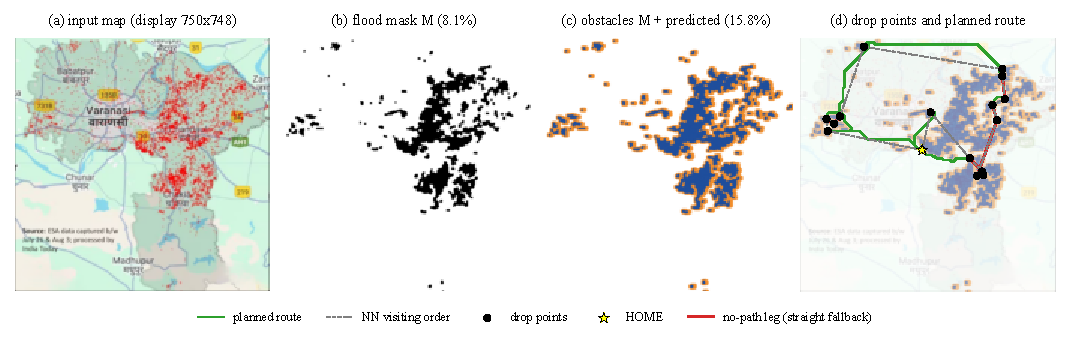
\includegraphics[width=0.92\textwidth]{figures/fig_pipeline.pdf}
\caption{Pipeline stages for the Varanasi map. (a) Input after display scaling (third-party map; see Data Availability). (b) Flood mask $M$. (c) Obstacles: $M$ (blue) and predicted-only pixels $\hat M\setminus M$ (orange). (d) Drop points, HOME, nearest-neighbour order (dashed), planned route (green) and the 8 no-path legs flown as straight segments (red).}
\label{fig:pipeline}
\end{figure*}

\subsection{Ablation: Predicted-Flood Obstacles}
Table~\ref{tab:ablation} and Fig.~\ref{fig:ablation} compare planning on $O=M\cup\hat M$ with planning on $M$ alone. Predicted-only pixels cover 7.7\% (Varanasi) and 14.0\% (Kanpur) of the image. Without predicted obstacles, 33.8\% and 47.9\% of the route length lies over predicted-only area. With them, exposure falls to 17.9\% and 11.6\%. Exposure does not reach zero because the no-path legs fly straight. The same inflation, however, causes \emph{all} no-path legs: there are none with $M$ alone, against 8 and 6 with $O$. It also increases planning time by a factor of 2.2--2.9, and for Varanasi it slightly increases exposure to the current flood (3.4\% to 4.8\%). The prediction stage is therefore not uniformly beneficial: in its current form, the benefit it is designed for comes with a loss of planner completeness.

\begin{table}[t]
\centering
\caption{Ablation of predicted-flood obstacles. Exposure is the share of route length over the given area.}
\label{tab:ablation}
\footnotesize
\setlength{\tabcolsep}{2.4pt}
\begin{tabular}{@{}llrrrrr@{}}
\toprule
Map & Obstacles & No-path & Items & Time (s) & \shortstack{Exposure\\pred.-only} & \shortstack{Exposure\\current}\\
\midrule
Varanasi & $M$ & 0 & 424 & 4.7 & 33.8\% & 3.4\%\\
 & $M\cup\hat M$ & 8 & 364 & 13.4 & 17.9\% & 4.8\%\\
Kanpur & $M$ & 0 & 733 & 16.5 & 47.9\% & 5.5\%\\
 & $M\cup\hat M$ & 6 & 1145 & 36.4 & 11.6\% & 4.3\%\\
\bottomrule
\end{tabular}
\end{table}

\begin{figure*}[t]
\centering
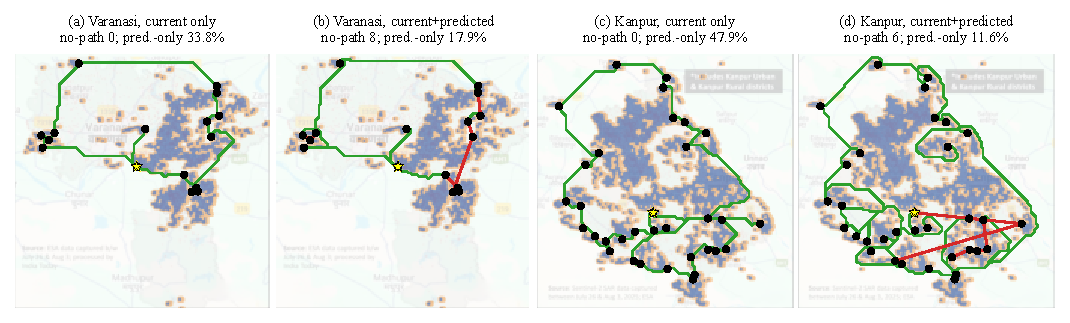
\includegraphics[width=0.92\textwidth]{figures/fig_ablation.pdf}
\caption{Planned routes with current-only obstacles (a, c) and with current and predicted obstacles (b, d). Blue: $M$; orange: $\hat M\setminus M$; red: no-path legs flown straight. Predicted obstacles move routes away from the predicted area but disconnect several drop points.}
\label{fig:ablation}
\end{figure*}

\subsection{Sensitivity}
Table~\ref{tab:sens} varies the colour margins and the number of operator clicks. The hue margin $\delta_H\in\{10,20,30\}$ has \emph{no} effect on any map, because the red-wrap rule replaces the hue interval. The saturation/value margin $\delta_{SV}\in\{15,30,45\}$ has a moderate effect on the two dot maps, while the Assam result is insensitive to every setting: its contamination is structural rather than a tuning artefact. Using 16 instead of 8 clicks raises the Varanasi flood fraction from 8.1\% to 9.7\% and the region count from 16 to 23, so the interactive step is a material source of variability. The ground scale $\rho$ affects only the geodetic conversion: the Varanasi route length scales linearly at 2.83~km per m/px, so the 5.66~km mission at $\rho=2$~m/px would be 263~km at the landmark-estimated scale of the map (Section~\ref{sec:geovalid}).

\begin{table}[t]
\centering
\caption{Sensitivity to the colour margin $\delta_{SV}$ and the number of clicks $K$ ($\delta_H=20$). Entries: flood-mask fraction (\%) / regions / no-path legs. Hue margins of 10, 20 and 30 give identical results.}
\label{tab:sens}
\footnotesize
\setlength{\tabcolsep}{3pt}
\begin{tabular}{@{}lccc@{}}
\toprule
Setting & Varanasi & Kanpur & Assam\\
\midrule
$\delta_{SV}=15$, $K=8$ & 7.2 / 19 / 8 & 14.0 / 32 / 6 & 83.1 / 1 / 0\\
$\delta_{SV}=30$, $K=8$ (default) & 8.1 / 16 / 8 & 15.1 / 33 / 6 & 83.1 / 1 / 0\\
$\delta_{SV}=45$, $K=8$ & 8.8 / 18 / 10 & 15.2 / 32 / 6 & 83.1 / 1 / 0\\
$\delta_{SV}=30$, $K=4$ & 8.1 / 16 / 8 & 15.1 / 33 / 6 & 83.1 / 1 / 0\\
$\delta_{SV}=30$, $K=16$ & 9.7 / 23 / 8 & 15.1 / 33 / 6 & 83.1 / 1 / 0\\
\bottomrule
\end{tabular}
\end{table}

\subsection{Route Ordering and Planner Baseline}
\label{sec:baselines}
Table~\ref{tab:baselines} reports two evaluation-only baselines; neither is part of \adapt{}. Against exact optima from Held--Karp dynamic programming \cite{held1962dynamic} on uniformly random instances, the nearest-neighbour order is on average 4.6\% (5 points) to 12.0\% (12 points) longer, with a worst case of 44.5\%. On the 16 Varanasi drop points it is 3.2\% longer than optimal. For the 33 Kanpur points only a minimum-spanning-tree lower bound is available, which limits the gap to at most 37.8\%.

The per-leg planner was compared with a plain grid A* \cite{hart1968formal} using the same grid, endpoints, costs and heuristic. The two agree on reachability for all 49 non-trivial legs and return equal path costs (difference below $2\times10^{-13}$), which supports the correctness of the D*~Lite implementation. As used in the pipeline, however, D*~Lite is 61 to 112 times slower than A*. Each leg builds a new instance and registers every obstacle cell, which amounts to 0.84 and 2.38 million vertex updates for the two maps, so its incremental design brings no benefit in this offline setting.

\begin{table}[t]
\centering
\caption{Evaluation-only baselines: route-ordering optimality and per-leg planner comparison.}
\label{tab:baselines}
\footnotesize
\setlength{\tabcolsep}{3pt}
\begin{tabular}{@{}lrrr@{}}
\toprule
\multicolumn{4}{@{}l}{\emph{Nearest neighbour / optimal tour length (random instances)}}\\
Points $n$ (instances) & Mean & Max & Optimal found\\
5 (300) & 1.046 & 1.257 & 42.3\%\\
8 (300) & 1.085 & 1.380 & 18.0\%\\
12 (100) & 1.120 & 1.445 & 11.0\%\\
Varanasi, $n=16$ & \multicolumn{3}{r}{1.032 (exact optimum)}\\
Kanpur, $n=33$ & \multicolumn{3}{r}{$\le$1.378 (MST bound)}\\
\midrule
\multicolumn{4}{@{}l}{\emph{Per-leg D*~Lite (as used) vs.\ grid A*, identical inputs}}\\
 & Varanasi & Kanpur & \\
Legs; reachability agreement & 16; 16/16 & 33; 33/33 & \\
Max.\ $|$cost difference$|$ & $4\times10^{-14}$ & $1\times10^{-13}$ & \\
Runtime D*~Lite / A* (s) & 12.67 / 0.21 & 30.83 / 0.28 & \\
\bottomrule
\end{tabular}
\end{table}

\subsection{Geospatial and Mission Verification}
\label{sec:verres}
Table~\ref{tab:verif} summarises the verification results; Fig.~\ref{fig:geodesy} shows resize consistency and model error. Every result in this subsection concerns \emph{software correctness}, that is, whether the code computes what its model specifies. None of it shows that the generated coordinates match real places.
\begin{itemize}
\item \emph{Synthetic ground truth.} On a $1000\times1000$~px synthetic image at 10~m/px, the implementation matches an independent re-derivation of \eqref{eq:enu}--\eqref{eq:geo} to within $1.4\times10^{-14}$~degrees at nine control points. Against the WGS84 geodesic ground truth, the largest error is 25.9~m at the image corners, dominated by the 0.49\% north--south scale error of $L$ at $25^\circ$, and every point is within the derived bound.
\item \emph{Round trips and edge cases.} Of 100\,000 randomised round trips through a test-only inverse, covering mid-latitudes, near-polar and near-antimeridian references, image sizes and scales from 0.05 to 633~m/px, 98\,789 are representable and agree within $6.8\times10^{-8}$~px; the remaining 1\,211 are correctly rejected.
\item \emph{Mission correspondence.} Every row of the three missions (1\,519 rows in total) matches an independent conversion of its source pixel within $3.6\times10^{-15}$~degrees. Traced back to the original image, the deviation is at most 0.57~m, entirely north--south and explained by the rounding of $H'$.
\item \emph{Resize consistency.} A synthetic three-region map run at nine display widths (300 to 2400~px, odd and even) yields drops at the same physical corners. They deviate from the model by at most one display pixel, and by $7\times10^{-10}$~m when no resizing occurs.
\item \emph{Mutation testing.} 22 of 24 injected defects are detected by the 126-test suite. The two surviving mutants are behaviour-equivalent: one removes a redundant finiteness guard, the other repeats a conversion.
\end{itemize}
During verification, the procedure exposed and led to the correction of defects in the original implementation: scale was not compensated after resizing, servo parameters were in the wrong slots, the region chosen as HOME received no delivery, the reference pixel was off by half a pixel, and invalid or polar inputs silently produced invalid coordinates. All results reported here use the corrected code.

\begin{table}[t]
\centering
\caption{Software verification of the geospatial and mission layers, and overall validation status.}
\label{tab:verif}
\footnotesize
\setlength{\tabcolsep}{3pt}
\begin{tabular}{@{}lr@{}}
\toprule
Check & Result\\
\midrule
\multicolumn{2}{@{}l}{\emph{Software correctness (performed)}}\\
Automated tests (incl.\ adversarial) & 126 + 494 subtests pass\\
Oracle vs.\ published geodesic & $\le$1 mm, $\le$0.01$''$\\
Implementation vs.\ model (synthetic) & $\le1.4\times10^{-14}$ deg\\
Model vs.\ WGS84, $\le$7.1 km offsets, 25$^\circ$ & $\le$25.9 m\\
Round trips (98\,789 compared) & max $6.8\times10^{-8}$ px\\
Mission rows vs.\ source pixels (1\,519) & $\le3.6\times10^{-15}$ deg\\
Resize, 9 display widths & $\le$1 display px\\
Mutants detected & 22/24 (2 equivalent)\\
Validator attack cases & 36 pass\\
Generated missions (3 maps) & 0 errors, 0 warnings\\
\midrule
\multicolumn{2}{@{}l}{\emph{Validation beyond software correctness}}\\
Geographic validity of supplied maps & not established\\
Ground-station load test (Mission Planner, QGC) & not performed\\
Software-in-the-loop (ArduPilot/PX4 SITL) & not performed\\
Hardware-in-the-loop / physical flight & not performed\\
\bottomrule
\end{tabular}
\end{table}

\begin{figure}[t]
\centering
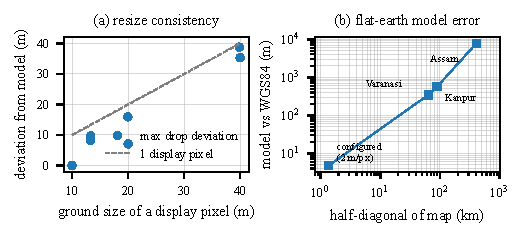
\includegraphics[width=\columnwidth]{figures/fig_geodesy.pdf}
\caption{(a) Maximum deviation of drop coordinates from the model across display widths, against the ground size of one display pixel. (b) Worst-case model error against WGS84 versus map half-diagonal: the configured 2~m/px setting and the landmark-estimated real extents of the three maps.}
\label{fig:geodesy}
\end{figure}

\subsection{Geographic Validity of the Supplied Maps}
\label{sec:geovalid}
To test whether the configured geography could describe the maps, a similarity transform was fitted between visible place-name labels and approximate public coordinates of those towns. This was done for 5, 10 and 12 labels on the Varanasi, Kanpur and Assam maps; the label positions were read off by eye. The estimate is a plausibility check, not a georeference. Residuals are 15--26~px and the rotations are $-0.5^\circ$, $-1.0^\circ$ and $-4.8^\circ$. The fitted scales are about 93, 130 and 633~m/px, which is 46, 65 and 317 times the configured 2.0~m/px. The default reference lies 23~km, 319~km and about 1\,000~km from the estimated image centres. At those extents, the flat-earth model itself would err by up to 345~m, 563~m and 7.7~km (Fig.~\ref{fig:geodesy}b), and the maps' web-Mercator basemaps violate the uniform-scale assumption \cite{battersby2014implications}. The generated missions are therefore \emph{not} geographically meaningful for these maps. The cause lies in the inputs and configuration, not in the conversion code.

\subsection{Mission Semantics}
The command parameters were audited against the MAVLink definitions and the ArduPilot and PX4 documentation \cite{mavlink_common,mavlink_mission,ardupilot_missioncmds,px4_missions}; the findings are given in Section~\ref{sec:method}-K and Section~\ref{sec:limits}. The lower block of Table~\ref{tab:verif} separates what has and has not been validated.

\section{Limitations, Threats to Validity and Safety}
\label{sec:limits}

\subsection{Limitations}
\emph{Geography.} The maps carry no georeferencing. The reference point $(\varphi_0,\lambda_0)$ is a command-line value whose default is Varanasi city for every map, and $\rho=2$~m/px is a configuration constant that is not derived from the image. Section~\ref{sec:geovalid} shows that both are wrong by one to two orders of magnitude for the supplied maps. Even with correct values, the conversion assumes north-up, square pixels of uniform scale, whereas web-Mercator basemaps change scale with latitude \cite{battersby2014implications}. The spherical constant $L$ introduces a scale error of up to 0.7\%, and the flat-earth approximation degrades over hundreds of kilometres (7.7~km at the Assam extent). The rounding of the display height adds an anisotropy of up to 0.06\%. Correcting it would require separate horizontal and vertical scales in the conversion, which is a change to the method.

\emph{Perception.} Segmentation extracts annotation colours from map products rather than detecting water in imagery. It depends on operator clicks and colour margins, and its accuracy is unknown because no ground-truth masks exist. On thematic maps with white backgrounds it can fail catastrophically (83\% flood for Assam). The hue margin is inert for red annotations.

\emph{Prediction.} The spread rule is a heuristic proxy, not a hydrological model \cite{teng2017flood}. It ignores terrain, drainage and flow, works in display pixels so that its physical reach depends on image resolution, rounds horizons down to whole hours, and treats Open-Meteo's current precipitation, which is a sum over the preceding reporting interval \cite{openmeteo_docs}, as an hourly rate. Its forecast skill has not been measured.

\emph{Selection and ordering.} Drop points are boundary vertices with no terrain, structure, population or landing-safety assessment. They are chosen relative to a centroid polyline in discovery order rather than to the final route, and they usually lie inside $O$ (98 endpoint snaps in the two dot maps). The ordering heuristic is up to 44.5\% longer than optimal in our random instances and ignores obstacles and vehicle endurance.

\emph{Planning.} The $5\times5$ nearest-neighbour downsampling inspects one pixel per block. Snapping can move endpoints into enclosed pockets, and the resulting no-path legs are flown straight across flooded or predicted areas (14 legs in our runs). D*~Lite is rebuilt per leg, so its incremental capability is unused and it is 61--112 times slower than A* on the same task. Routes depend on display width because the grid cell is defined in display pixels.

\emph{Mission design.} The servo is set to 2000~$\mu$s at every drop and never reset, so a release mechanism that requires a toggle would release only once. LAND after RTL is redundant on ArduCopter \cite{ardupilot_missioncmds}. Waypoint yaw 0 would point a PX4 vehicle north at every waypoint \cite{px4_missions}. Servo channel 9 and the 100/10~m altitudes are assumptions, and altitudes are relative to home without terrain following. Mission length is not checked against the flight controller's mission capacity, which matters for missions with more than 1\,000 items such as Kanpur's. The route length is not checked against vehicle endurance; at the estimated real scale of Varanasi it would be 263~km.

\subsection{Threats to Validity}
\emph{Internal validity.} Correctness evidence is strongest for the geospatial and mission layers, which were verified against an independent oracle and a validator that were themselves tested and mutation-checked. The perception, prediction and planning stages are evaluated behaviourally, not against ground truth. All experiments use a single simulated operator and a single weather setting, so operator and weather variability are only partly explored by the sensitivity study. With calm weather the predicted mask equals $M$, so the ablation's current-only condition also describes that case. Runtimes are single measurements on one machine.

\emph{Construct validity.} Route exposure measures geometric overlap with masks, not risk to the vehicle or to people. ``No-path legs'' and ``validator errors'' measure planner completeness and format conformance, not mission success. The landmark-based scale estimate is a plausibility check whose label positions were read off by eye.

\emph{External validity and dataset validity.} The three maps are convenience samples of one style of news graphic and one thematic map, all from India; they are not a benchmark. Their copyright belongs to third parties, and the actual flood observations behind them are not available. The results cannot be generalised to UAV or satellite imagery, to other annotation colours, or to other regions.

\emph{Literature coverage.} The review was targeted rather than systematic: candidates were identified by keyword searches and verified against DOI registries. Statements that a capability is ``not reported'' are therefore bounded by the reviewed set.

\emph{Geographic validity.} For the supplied maps, the generated coordinates do not correspond to the flooded places (Section~\ref{sec:geovalid}). The conversion is correct for correctly specified inputs; obtaining such inputs is outside the current system.

\emph{Operational validity.} Mission semantics were checked against documentation only. No ground station has loaded the missions, and no SITL, HITL or flight test has been performed, so the behaviour of a real autopilot and vehicle is unverified.

\emph{Reproducibility.} The code, inputs, evaluation scripts and raw results are versioned with the paper, and all experiments are deterministic except runtimes. Python dependency versions are recorded but not pinned in the project's requirements, which may affect future reproduction.

\subsection{Safety and Operational Considerations}
\adapt{} is \emph{not} flight-ready and must not be used to fly over people or property. Any operational use would require, at minimum: georeferenced inputs and an independent check of every coordinate against base maps; a ground-station load and SITL rehearsal of the exact mission; geofences, altitude limits and failsafes for link loss, battery and GNSS degradation configured on the autopilot; a trained pilot able to take control; verification that drop points are clear of people, structures and water hazards; a payload-release mechanism tested on the ground with the configured channel and PWM; and compliance with local aviation regulations. The software design supports some of these practices: it rejects invalid coordinates before writing a file, it never leaves a partial or stale mission at the output path, and it logs every no-path leg so that an operator can inspect straight segments before flight. It cannot, however, detect that a valid-looking coordinate is in the wrong place.

\section{What \adapt{} Offers Relative to Prior Work}
\label{sec:compare}

Table~\ref{tab:gap} shows that \adapt{} covers more stages of the image-to-mission chain than any single group of reviewed works. This breadth is its main contribution, and it comes with explicit trade-offs.

\emph{End-to-end executable output.} Flood-mapping methods \cite{twele2016sentinel,gebrehiwot2019deep,simantiris2024unsupervised} end at a mask, and relief-routing models \cite{rabta2018drone,dong2026path} end at a schedule over given nodes. \adapt{} produces a file that MAVLink ground stations are designed to load, containing explicit delivery actions. The trade-off is that each stage is simpler than its specialised counterpart: colour thresholding instead of learned or spectral segmentation, a heuristic spread rule instead of a hydrodynamic or CA inundation model \cite{jamali2019cellular}, a nearest-neighbour heuristic instead of exact or metaheuristic optimisation, and boundary geometry instead of site-safety scoring \cite{patterson2014timely}.

\emph{Low data and compute requirements.} The pipeline needs no training data, no digital elevation model and no GPU. It runs on a laptop in under 40~s for the evaluated maps, with planning taking almost all of that time; on these inputs a static A* planner would reduce planning to under 0.3~s (Table~\ref{tab:baselines}). The price is that nothing in the pipeline is calibrated against physical flood behaviour or delivery safety.

\emph{Weather-informed obstacles.} Unlike static-map planners \cite{aggarwal2020path}, \adapt{} inflates obstacles according to current precipitation and wind. Our ablation shows that this reduces the route length over predicted flooding by 47\% and 76\% on the two dot maps, but disconnects drop points that the planner then reaches by straight, unchecked legs. Prior CA flood models are physically richer but are not coupled to planning \cite{ghimire2013formulation,guidolin2016weighted}.

\emph{Verified geospatial and mission layers.} We found no reviewed image-to-UAV-mission work that reports independent verification of its coordinate conversion and mission encoding. \adapt{} provides an independent geodetic oracle, a tested validator and mutation evidence, and states the conversion's validity domain. This strengthens confidence in the software, but it does not substitute for geographic validation of the inputs or for flight testing. Because code, evaluation scripts and results are released together, any component (for example a learned segmenter or a CA flood model) can be replaced and re-evaluated in place.

\section{Future Work}
\label{sec:future}
Future work follows directly from the limitations, roughly in order of cost:
\begin{enumerate}
\item \emph{Operational validation.} Load the generated missions in Mission Planner and QGroundControl, then execute them in ArduPilot and PX4 SITL to confirm item acceptance, servo timing, RTL behaviour and mission-storage limits, before any hardware-in-the-loop or field trial.
\item \emph{Georeferenced inputs.} Accept georeferenced rasters (for example GeoTIFF flood products from SAR processing chains \cite{twele2016sentinel}) or ground control points, replace the single scale with an affine or projective georeference, and treat web-Mercator inputs with the correct projection \cite{battersby2014implications,snyder1987map}.
\item \emph{Segmentation ground truth.} Annotate the evaluation maps, report IoU, precision and recall, and evaluate on public benchmarks such as FloodNet and Sen1Floods11 \cite{rahnemoonfar2021floodnet,bonafilia2020sen1floods11}.
\item \emph{Planner completeness.} Detect disconnected drop points and handle them explicitly, for example by reporting them, selecting another boundary vertex, or planning only on current flooding, instead of flying straight legs. Plan at a resolution defined in metres, and either exploit D*~Lite's incremental reuse during flight or use a static planner offline.
\item \emph{Prediction.} Calibrate or replace the spread rule with terrain-aware CA models \cite{guidolin2016weighted,jamali2019cellular}, and use precipitation accumulations with explicit time bases.
\item \emph{Mission and logistics.} Add endurance and payload constraints, better ordering heuristics or exact methods for small instances, multi-UAV allocation \cite{otto2018optimization,dong2026path}, and site-safety scoring for drop points \cite{patterson2014timely,kaljahi2019automatic}.
\end{enumerate}

\section{Conclusion}
\label{sec:conclusion}
This paper presented \adapt{}, an open pipeline that converts a flood-annotated map raster and current weather into a QGroundControl WPL~110 UAV relief mission. It combines colour-based flood extraction, a weather-driven obstacle-inflation rule, boundary drop-point selection, nearest-neighbour ordering, per-leg D*~Lite planning and a flat-earth geodetic conversion with explicit validity checks. It offers two approaches. Either one drone visits every drop point, or a fleet of drones is used, in which each drone serves the cluster of drop points around its own launch base under a battery and payload model. Fleet plans whose routes cross are rejected. The work addresses an intersection that the reviewed literature treats in separate pieces. Its contribution is integration and verification rather than any individual algorithm.

On three published flood maps the pipeline produced missions with 16, 33 and 1 deliveries, all of which passed an independent specification-based validator. The geospatial and mission layers were verified against an independent WGS84 oracle: mission rows match their source pixels within $3.6\times10^{-15}$~degrees, 98\,789 randomised round trips agree within $7\times10^{-8}$~px, and 31 of 33 injected defects were detected. With identical inputs, the multi-base mode reproduced its reference implementation's plans exactly. In the fleet runs, 190 of 206 served flood regions went to a single drone, so each drone in effect took its own cluster. Raising the number of bases from one to four increased the drops served from 10 to 18 of 22 (Varanasi) and from 17 to 34 of 41 (Kanpur) under moderate weather. All 43 resulting missions passed the validator, and no routes crossed. Because the assignment does not balance work, however, one Kanpur base kept 15 to 17 drops throughout. The same evaluation exposed limits of the approach. Predicted-flood obstacles reduce the route's exposure to predicted flooding by 47\% and 76\%, but cause all 14 no-path legs, which are flown as straight segments. Segmentation of a thematic map labels 83\% of it as flood. The nearest-neighbour order is up to 44.5\% longer than optimal on random instances. The per-leg D*~Lite is 61--112 times slower than A* because its incremental reuse is unused. Finally, the supplied maps are not georeferenced and their configured scale is wrong by factors of 46--317, so the generated coordinates are not geographically meaningful.

\adapt{} is therefore best understood as a verified software baseline for image-to-mission research, not as a deployable system. The most important next steps are ground-station and SITL validation of both modes, georeferenced inputs, segmentation ground truth, explicit handling of disconnected drop points in the single-UAV mode, and workload-aware, temporally deconflicted multi-UAV allocation.

\section*{Data Availability}
The \adapt{} source code, test suite, evaluation scripts (\texttt{paper/experiments}), raw results (\texttt{paper/experiments/results}) and figure generators are available at [REPOSITORY URL --- to be provided by the authors; an archived DOI, e.g.\ Zenodo, is recommended]. The three input maps are third-party graphics reproduced from published sources. The authors must confirm redistribution rights before public release, or replace them with openly licensed georeferenced flood products. No ground-truth flood masks, georeferences or flight logs exist for these inputs.

\section*{Acknowledgment}
[Funding and institutional acknowledgments --- to be provided by the authors.] In accordance with IEEE policy on AI-generated content, the authors disclose the following use of an AI system (Anthropic Claude, model Claude Opus 5.5, accessed through the Claude Code tool):
\begin{itemize}
\item drafting of all sections of this manuscript and of the figure, table and bibliography generation scripts;
\item writing of the evaluation scripts in \texttt{paper/experiments} and of parts of the verification test suite;
\item the code review that identified and corrected the implementation defects listed in Section~\ref{sec:verres}.
\end{itemize}
All experiments were executed on the authors' machine, and every reported number is traceable to a result file in the repository. The authors are responsible for reviewing and verifying all content before submission. [Authors: state the extent of your own review and edits here.]


\bibliographystyle{IEEEtran}
\bibliography{references}

\end{document}
